\section{Analog-til-digital konvertering (ADC)}\label{sec:ADC}
En analog til digital konverter kan anvendes til at konvertere et sammenhængende analogt spændingssignal til et diskret digitalt nummer. TMC4C123GH6PM microcontrolleren har to identiske 12 bit A/D konvertere indbygget - ADC0 og ADC1. Det konverterede signal, kan derefter behandles vha. digitale signalbehandlingsmetoder. 
Da der ønskes at opbygge en stereostyret equalizer, bruges begge A/D konvertere. Konfigurationen er derfor ens på hhv. ADC0 og ADC1. Begge A/D konvertere kører uafhængigt af hinanden. Afhængig af hvilken Sample frequencer der er valgt, gemmes
resultatet af A/D konverteringen i et FIFO register (first in - first out). Da der kun er brug for én sample ad gangen, vælges ud fra databladet at konfigurere A/D konverterne med Sample sequencer 3, og derved gemmes resultatet af konverteringen også i ADCSSFIFO3 registeret for hhv. ADC0 og ADC1.
Da det ikke er alle porte, der kan anvendes på microcontrolleren til A/D konvertering, er pin PB5 valgt til at styre venstre kanal, og pin PE4 er valgt til at styre højre kanal. Herudover kan den også køre i mono, frem for stereo - denne er konfigureret på pin PE5. Der ønskes en samplingsfrekvens på $44,1\si\kilo\hertz$ for at undgå aliasing. Denne samplingsfrekvens er bestemt ud fra Nyquist frekvensen. For at få denne samplingsfrekvens korrekt, skal microcontrollerens CPU frekvens sættes til $80\si\mega\hertz$. Der bruges et PWM signal, som er interruptstyret. Dette signal skal køre et bestemt antal cycles.

 \begin {equation}
 \text{Cycles} = \frac{\text{CPU frekvens}}{\text{Sample frekvens}} => \frac{80\cdot 10^6\si\hertz}{44100\si\hertz} = 1814 \text{cycles}
 \end {equation}

Hver gang PWM'en har kørt i det beregnede antal cycles, bliver et interrupt initialiseret, og samplingen starter samt gemmer værdien. Ved næste interrupt, starter processen for A/D konverteringen igen.
Da A/D konverterne har en opløsning i 12 bit, og den maksimale spænding der bliver registreret er $3,3\si\volt$ - vil maksimalværdien for konverteringen være $4096$. Flowchartet af dette forløb, kan ses på figur \ref{fig:ADC}.
\begin{figure}[h]
	\centering

		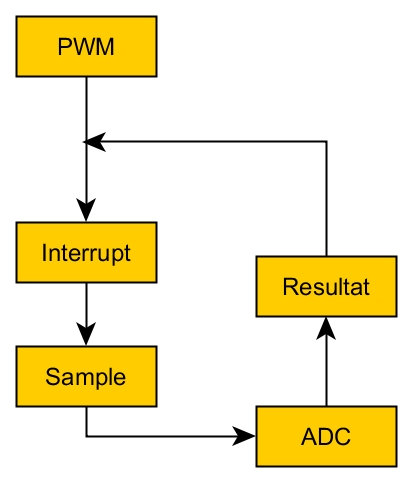
\includegraphics[width=.6\textwidth]{billeder/ADC.jpg}
			
	
	\caption{Flowchart der beskriver forløbet af A/D konverteringen.}
	\label{fig:ADC}
\end{figure}



